\section{Geometric models: wave maps and relativistic membranes}
\label{geom:sec}

This section treats two \emph{geometric} wave equations: the wave map
($\sigma$-model) equation, which is semilinear and for which the Donninger
programme is essentially complete, and the timelike minimal-surface
(Nambu--Goto, scalar Born--Infeld) equation, which is quasilinear and for
which it is not. Throughout we separate
\textbf{(K)} known results (with references),
\textbf{(D)} what is derived or computed here (scripts
\texttt{code/geom\_*.py}), and
\textbf{(C)} conjectural statements.

\subsection{Wave maps: origin, scaling, and what is industrially relevant}
\label{geom:sec:wm-origin}

A wave map $\bm u:\mathbb{R}^{1+d}\to S^m\subset\mathbb{R}^{m+1}$ is a
critical point of $\frac12\int(|\partial_t\bm u|^2-|\nabla\bm u|^2)$ under
the constraint $|\bm u|=1$:
\begin{equation}\label{geom:eq:wm}
  \partial_t^2\bm u-\Delta\bm u=\bigl(|\nabla\bm u|^2-|\partial_t\bm u|^2\bigr)\bm u .
\end{equation}
\emph{Where it comes from.} (a) In the Ericksen--Leslie theory of nematic
liquid crystals with director inertia $\sigma_1$, one-constant Frank energy
$K$, frozen flow and no dissipation, the director $\bm n\in S^2$ obeys
\eqref{geom:eq:wm} with wave speed $c^2=K/\sigma_1$; unequal elastic
constants lead to the variational wave equations of Hunter and
Saxton~\cite{HunterSaxton1991}. (b) Inertial magnetisation dynamics
(nutation) has been observed in ferromagnetic films at sub-THz
frequencies~\cite{NeerajEtAl2021}; in antiferromagnets the leading-order
dynamics of the N\'eel vector is a nonlinear $\sigma$-model, i.e.\ a wave map
into $S^2$. % TODO verify: add a reference (Andreev--Marchenko / Haldane)
(c) In physics, the $O(4)$ $\sigma$-model ($m=3$, $d=3$) describes
cosmological textures; its collapse is the explicit self-similar solution of
Shatah~\cite{Shatah1988} and Turok--Spergel~\cite{TurokSpergel1990}.

\emph{Honest assessment.} In display-type liquid crystals the director
motion is overdamped and $\sigma_1$ is negligible, so \eqref{geom:eq:wm} is
a formal inertial limit. A damping term $\gamma\,\partial_t\bm u$ is, however,
a lower-order perturbation in similarity variables (relative size
$\gamma(T-t)$, cf.\ \cref{fw:subsec-lower}): \emph{if} a
singularity forms in the inertial regime, damping is asymptotically
irrelevant, and the inertial self-similar regime is entered only when
$T-t\ll\sigma_1/\gamma$. The scaling $\bm u\mapsto\bm u(\mu t,\mu x)$ ($s=0$)
leaves \eqref{geom:eq:wm} invariant and multiplies the energy by
$\mu^{2-d}$, so $d=2$ is energy critical and $d\ge3$ supercritical.
\begin{itemize}[leftmargin=*]
\item $d=2$ (films, planar magnets; target $S^2$): there is no
  self-similar blowup; energy cannot concentrate in the interior of the
  backward light cone \textbf{(K)}~\cite{ShatahTahvildarZadeh1992}, and
  equivariant blowup happens by bubbling off a harmonic map
  \cite{Struwe2003}, at non-self-similar (type~II) rates constructed in
  \cite{KriegerSchlagTataru2008} and shown to be stable within
  co-rotational symmetry in \cite{RaphaelRodnianski2012}. Donninger's
  method is \emph{not} the right tool there.
\item $d=3$, target $S^3$: self-similar blowup is generic and stable
  (\cref{geom:sec:wm-thm}). For the physically most relevant case
  \emph{$d=3$, target $S^2$} (bulk nematics, magnets) the co-rotational
  reduction below is unavailable; self-similar wave maps can still be
  sought as harmonic maps from hyperbolic space
  \cite{CazenaveShatahTahvildarZadeh1998}, but we are not aware of a
  stability theory for $S^2$ targets. What transfers is the method
  (similarity variables, mode stability without symmetry as in
  \cite{WeissenbacherKochDonninger2025,DonningerMoscatelli2026a}); what
  does not transfer is the explicit profile.
\end{itemize}

\subsection{Co-rotational wave maps and similarity variables}
\label{geom:sec:wm-setup}

For $m=d$ and the co-rotational ansatz
$\bm u(t,x)=(\sin u(t,r)\,\tfrac{x}{r},\cos u(t,r))$, $r=|x|$,
\eqref{geom:eq:wm} becomes
\begin{equation}\label{geom:eq:corot}
  u_{tt}-u_{rr}-\frac{d-1}{r}u_r+\frac{d-1}{2r^2}\sin(2u)=0 .
\end{equation}
\begin{proposition}[\textbf{K}; verified \textbf{D}]\label{geom:prop:profile}
For $d\ge3$, $u_T(t,r)=f_0\!\bigl(\frac{r}{T-t}\bigr)$ with
$f_0(\rho)=2\arctan\bigl(\rho/\sqrt{d-2}\bigr)$ solves \eqref{geom:eq:corot};
equivalently $f_0$ solves
$(\rho^2-1)f''+(2\rho-\tfrac{d-1}{\rho})f'+\tfrac{d-1}{2\rho^2}\sin 2f=0$
and is analytic on $[0,\infty)$, in particular across the light cone $\rho=1$.
\end{proposition}
This is due to Shatah and Turok--Spergel for $d=3$ and to
Bizo\'n--Biernat~\cite{BizonBiernat2015} for $d\ge4$; we checked it
symbolically for $3\le d\le 10$ (\texttt{geom\_wavemaps\_symbolic.py}).
For $d=3$, $f_0$ is the ground state of a family of smooth self-similar
solutions; numerically it attracts generic large data, and the first excited
one, which has exactly one unstable mode, sits at the threshold of blowup
\cite{BizonChmajTabor2000}.

\emph{Reduction to a semilinear radial equation.} Writing $u=r\psi$,
\eqref{geom:eq:corot} becomes (checked symbolically)
\begin{equation}\label{geom:eq:psi}
  \psi_{tt}-\Delta_{\mathbb{R}^{d+2}}\psi
  +\frac{d-1}{2r^3}\bigl(\sin(2r\psi)-2r\psi\bigr)=0,
\end{equation}
a radial wave equation on $\mathbb{R}^{d+2}$ with a smooth nonlinearity and
scaling exponent $s=1$. With $\psi_1=(T-t)\psi$, $\psi_2=(T-t)^2\psi_t$ and
$\xi\in\mathbb{B}^{d+2}$, the conventions of \cref{fw:sec} give an
\emph{autonomous} system, because
$(T-t)^3\frac{d-1}{2r^3}(\sin 2r\psi-2r\psi)
=\frac{d-1}{2|\xi|^3}(\sin 2|\xi|\psi_1-2|\xi|\psi_1)$.
The profile is $\psi_1=f_0(|\xi|)/|\xi|$. Linearising,
$\partial_\tau\Phi=(\mathbf L_0+\mathbf L')\Phi$ with
$\mathbf L'(\phi_1,\phi_2)=(0,-V\phi_1)$ and
\begin{equation}\label{geom:eq:V}
  V(\rho)=\frac{(d-1)(\cos 2f_0(\rho)-1)}{\rho^2}
         =-\frac{8(d-1)(d-2)}{(d-2+\rho^2)^2}\qquad(V=-\tfrac{16}{(1+\rho^2)^2}\text{ for }d=3).
\end{equation}
$\mathbf L'$ is compact on radial $\mathcal H_k:=H^k\times H^{k-1}(\mathbb{B}^{d+2})$.
For the free operator, the known Lumer--Phillips estimates (e.g.\
\cite{Donninger2011,ChatzikaleasDonningerGlogic2017,Glogic2025}) give a
growth bound $-\omega_k$ which, by scaling, should have
$\omega_k=k-\frac{d+2}{2}+1=k-\frac d2$ (the decay rate of \cref{fw:sec} with $s=1$
in dimension $d+2$).
\textbf{(D)} This value is sharp: for $\operatorname{Re}\lambda<-\omega_k$ both Frobenius branches at $\rho=1$,
$1$ and $(1-\rho^2)^{\frac{d-1}{2}-\lambda}$, lie in $H^k$ near $\rho=1$
(the second iff $\frac{d-1}{2}-\operatorname{Re}\lambda>k-\frac12$), so the
free mode regular at $\rho=0$ is an eigenfunction in $\mathcal H_k$ and every such
$\lambda$ is in the spectrum. Hence the spectrum of
$\mathbf L$ in $\{\operatorname{Re}\lambda>\frac d2-k\}$ consists of isolated
eigenvalues, and the regularity $k$ determines how much of it is visible.

\subsection{The spectral problem and how mode stability is proved}
\label{geom:sec:wm-spec}

Modes of the linearisation of \eqref{geom:eq:psi},
$\delta\psi=(T-t)^{-1-\lambda}g(\rho)$ (equivalently
$u-u_T\propto(T-t)^{-\lambda}\rho\,g(\rho)$, with the same $\lambda$), solve
\begin{equation}\label{geom:eq:mode}
  (1-\rho^2)g''+\Bigl(\frac{d+1}{\rho}-2(\lambda+2)\rho\Bigr)g'
  -(\lambda+1)(\lambda+2)g-V(\rho)g=0,\qquad 0<\rho<1 .
\end{equation}
The Frobenius exponents are $\{0,-d\}$ at $\rho=0$ and
$\{0,\sigma_2\}$, $\sigma_2=\frac{d-1}{2}-\lambda$, at $\rho=1$. We call
$\lambda$ an \emph{eigenvalue} if \eqref{geom:eq:mode} has a nonzero solution
in $C^\infty[0,1]$; for $\operatorname{Re}\lambda>\frac d2-k$ this coincides
with the eigenvalues of $\mathbf L$ on $\mathcal H_k$. Generically the
condition at $\rho=1$ excludes the $(1-\rho)^{\sigma_2}$ branch; when
$\sigma_2\in\mathbb N$ the exponent-$0$ branch may carry a logarithm, and if it
does not, the point $\rho=1$ imposes no condition at all.

\emph{Symmetry mode.} Time translation gives
$\partial_T u_T=-(T-t)^{-1}\rho f_0'(\rho)$, i.e.\ $\lambda=1$ with
$g_1=f_0'\propto(d-2+\rho^2)^{-1}$ (checked). Space translations and
Lorentz boosts leave the co-rotational class and appear only in the
non-symmetric problem. \emph{Mode stability} means: no eigenvalue with
$\operatorname{Re}\lambda\ge0$ except $\lambda=1$. The instability $\lambda=1$
is removed in the nonlinear argument by adjusting the blowup time $T$.

\begin{proposition}[Hyperbolic reformulation; \textbf{D}]\label{geom:prop:hyp}
Put $\rho=\tanh\eta$, $g=\cosh^{1+\lambda}(\eta)\,\chi(\eta)$,
$\kappa=\lambda-\frac{d-1}{2}$ and
$\psi_{\mathrm{1D}}=\sinh^{\frac{d+1}{2}}(\eta)\,\chi$. Then
\eqref{geom:eq:mode} is equivalent to
\begin{equation}\label{geom:eq:H}
  \Bigl(-\Delta_{\mathbb H^{d+2}}-\tfrac{(d+1)^2}{4}+W\Bigr)\chi=-\kappa^2\chi
  \iff
  H\psi_{\mathrm{1D}}:=-\psi_{\mathrm{1D}}''+Q\,\psi_{\mathrm{1D}}=-\kappa^2\psi_{\mathrm{1D}},
\end{equation}
with $W(\eta)=V(\tanh\eta)/\cosh^2\eta$ and
$Q=\frac{(d+1)(d-1)}{4\sinh^2\eta}+W$, a self-adjoint operator on
$L^2(0,\infty)$ \emph{independent of $\lambda$}. Smoothness of $g$ at
$\rho=1$ means $\psi_{\mathrm{1D}}=e^{-\kappa\eta}F(e^{-2\eta})$ with $F$
analytic at $0$, i.e.\ $\psi_{\mathrm{1D}}$ is the (analytically continued)
Jost solution.
\end{proposition}
\begin{proof}[Sketch]
Inside the backward light cone write $T-t=e^{-\sigma}\cosh\eta$,
$r=e^{-\sigma}\sinh\eta$; then the Minkowski metric equals
$e^{-2\sigma}(-d\sigma^2+g_{\mathbb H^{d+2}})$. Conformal covariance of the
conformal wave operator in dimension $d+3$, with scalar curvature
$-(d+2)(d+1)$ of $\mathbb H^{d+2}$, turns
$\psi_{tt}-\Delta\psi+V(\rho)(T-t)^{-2}\psi=0$ into
$\varphi_{\sigma\sigma}-\Delta_{\mathbb H}\varphi-\frac{(d+1)^2}{4}\varphi+W\varphi=0$
for $\varphi=e^{-\sigma(d+1)/2}\psi$; a mode is $\varphi=e^{\kappa\sigma}\chi(\eta)$.
We verified the resulting identity for \eqref{geom:eq:mode} symbolically and
at random complex $\lambda$ (\texttt{geom\_wavemaps\_symbolic.py}).
\end{proof}
\noindent\emph{Consequences.} (i) If $\operatorname{Re}\lambda>\frac{d-1}{2}$
then $\psi_{\mathrm{1D}}\in L^2$, so $-\kappa^2$ is an eigenvalue of $H$ and
$\lambda$ is \emph{real}; on $\operatorname{Re}\kappa=0$, $\kappa\neq0$ the Jost
function does not vanish. For $d=3$ the zero-energy solution regular at
$\eta=0$ is the gauge mode itself,
$\psi_{\mathrm{1D}}=\sinh^2\eta/\cosh2\eta>0$ (a threshold resonance), so
$H\ge0$ by Sturm's theorem: \emph{no eigenvalue with $\operatorname{Re}\lambda\ge1$
other than $\lambda=1$}. For $d\ge4$ the gauge mode is a positive solution of
$H\psi=-\kappa_1^2\psi$, $\kappa_1=\frac{3-d}{2}$, whence $H\ge-\kappa_1^2$
(Allegretto--Piepenbrink) and there are no eigenvalues $\lambda>d-2$; for
$\frac{d-1}{2}<\lambda\le d-2$ we counted the nodes of the zero-energy
solution numerically (none for $4\le d\le8$). (ii) In the strip
$0\le\operatorname{Re}\lambda<\frac{d-1}{2}$ the eigenvalues are
\emph{resonances} of $H$ (zeros of the continued Jost function with
$\operatorname{Re}\kappa<0$); no self-adjointness argument applies, and this is
where the difficulty of mode stability lies. For $d\ge4$ the gauge mode lies
inside this strip.

\begin{proposition}[Supersymmetric removal of the gauge mode; \textbf{D}]\label{geom:prop:susy}
Let $\psi_\star=\sinh^{\frac{d+1}{2}}\eta\,/\bigl((d-2)\cosh^2\eta+\sinh^2\eta\bigr)>0$
(the gauge mode) and $w=-\psi_\star'/\psi_\star$. Then
$H+\kappa_1^2=(-\partial_\eta+w)(\partial_\eta+w)$, and the partner
$\widetilde H=(\partial_\eta+w)(-\partial_\eta+w)-\kappa_1^2=H+2w'$ is, after
the substitutions of \cref{geom:prop:hyp} read backwards with $d+4$ in place of
$d+2$ and $\lambda+1$ in place of $\lambda$, the mode problem
\begin{equation}\label{geom:eq:susy}
  (1-\rho^2)h''+\Bigl(\frac{d+3}{\rho}-2(\lambda+3)\rho\Bigr)h'
  -(\lambda+2)(\lambda+3)h+\frac{4(d-1)}{d-2+\rho^2}\,h=0 .
\end{equation}
The intertwiner $\partial_\eta+w$ maps smooth modes of \eqref{geom:eq:mode}
to smooth modes of \eqref{geom:eq:susy} and annihilates the gauge mode; since
$(-\partial_\eta+w)(\partial_\eta+w)=\kappa_1^2-\kappa^2$ on modes, it is
injective for $\lambda\notin\{1,d-2\}$, and $\lambda=d-2$ is an eigenvalue of
neither problem. Hence
$\operatorname{spec}\eqref{geom:eq:susy}=\operatorname{spec}\eqref{geom:eq:mode}\setminus\{1\}$,
and mode stability is equivalent to the absence of eigenvalues of
\eqref{geom:eq:susy} with $\operatorname{Re}\lambda\ge0$.
\end{proposition}
The partner potential $-4(d-1)/(d-2+\rho^2)$ was found and checked
symbolically for $3\le d\le8$; the numerical spectra of
\eqref{geom:eq:mode} and \eqref{geom:eq:susy} agree to 20 digits except for
$\lambda=1$ (\cref{geom:tab:spec}). Removing the gauge mode by a Darboux
transformation in this spirit is the standard first step in the rigorous
proofs; we have not checked whether the cited works use exactly this
partner.
% TODO verify: compare with the transformation used in CostinDonningerXia2016 / CostinDonningerGlogic2017.

\emph{How the remaining strip is handled (K).} Donninger--Aichelburg
excluded real unstable eigenvalues other than $\lambda=1$
\cite{DonningerAichelburg2008}; Donninger--Sch\"orkhuber--Aichelburg
confined possible unstable eigenvalues to a compact set
\cite{DonningerSchoerkhuberAichelburg2012}; Costin--Donninger--Xia proved
mode stability for $d=3$ \cite{CostinDonningerXia2016} and
Costin--Donninger--Glogi\'c for all $d\ge4$ \cite{CostinDonningerGlogic2017}.
In outline (as we understand it), the \emph{quasi-solution method} of the
latter works with the power series of the solution regular at the origin
(after removal of the gauge mode): $\lambda$ is an eigenvalue iff that series
converges beyond $\rho=1$. The coefficients satisfy a finite-term
recurrence; one writes down an explicit approximate solution (the
quasi-solution) for the ratio of consecutive coefficients and controls the
error rigorously, showing that the ratio tends to $1$ for all
$\operatorname{Re}\lambda\ge0$. The radius of convergence is then $1$, and if
$\rho=1$ is the only singular point of the equation on the unit circle, the
solution must be singular there. \emph{Observation (D):} this last step is
where $d=3$ differs: the potential \eqref{geom:eq:V} has poles at
$\rho=\pm i$, on the unit circle, whereas for $d\ge4$ the poles
$\pm i\sqrt{d-2}$ lie outside it (the same holds for the partner
potential in \eqref{geom:eq:susy}).

\subsection{Numerically computed spectrum}
\label{geom:sec:wm-num}

We used three independent methods (\texttt{geom\_modes.py},
\texttt{geom\_wavemaps\_spectrum.py}): (1) Chebyshev collocation in
$y=\rho^2$ with $N=40,\dots,120$ nodes, without boundary conditions (both ends
are singular points), linearising the quadratic pencil; (2) Frobenius series
about $y=0$ and $y=1$ (400 terms, 30--35 digits), whose Wronskian at
$y=\frac12$, multiplied by $1/\Gamma(1-\sigma_2)$, is an \emph{entire}
function of $\lambda$ whose zeros are exactly the eigenvalues (the factor
removes the poles at $\sigma_2\in\mathbb N$, and log-free resonances are zeros
automatically), refined by Newton's method; (3) the argument principle for
this Wronskian on the rectangle
$[-1.9,4]\times[-15,15]$ ($1200$ points, maximal phase step $<0.6$\,rad).
\begin{table}[ht]
\centering\footnotesize
\begin{tabular}{@{}llll@{}}
\toprule
 & $d=3$ & $d=4$ & $d=5$\\
\midrule
gauge & $1$ & $1$ & $1$\\
$\lambda_1$ & $-0.54246\,63534\,31726\,5370$ & $-0.56361\,26748\,07079\,4374$ & $-0.57231\,57218\,74117\,6664$\\
$\lambda_2$ & $-2$ (exact) & $-2.10913\,10073\,42525\,1316$ & $-2.16301\,19522\,28281\,9288$\\
winding \eqref{geom:eq:mode}/\eqref{geom:eq:susy} & $2\,/\,1$ & $2\,/\,1$ & $2\,/\,1$\\
\bottomrule
\end{tabular}
\caption{Eigenvalues of \eqref{geom:eq:mode} with $\operatorname{Re}\lambda\ge-2.2$
(Wronskian method; digits stable under changes of truncation and precision).
Collocation reproduces $\lambda_1$ to $10^{-8}$ for $N=40$--$80$ (round-off
grows for larger $N$). The last row is the winding number of the Wronskian on
$[-1.9,4]\times[-15,15]$ for the original and the SUSY-partner problem.}
\label{geom:tab:spec}
\end{table}

\begin{figure}[ht]
\centering
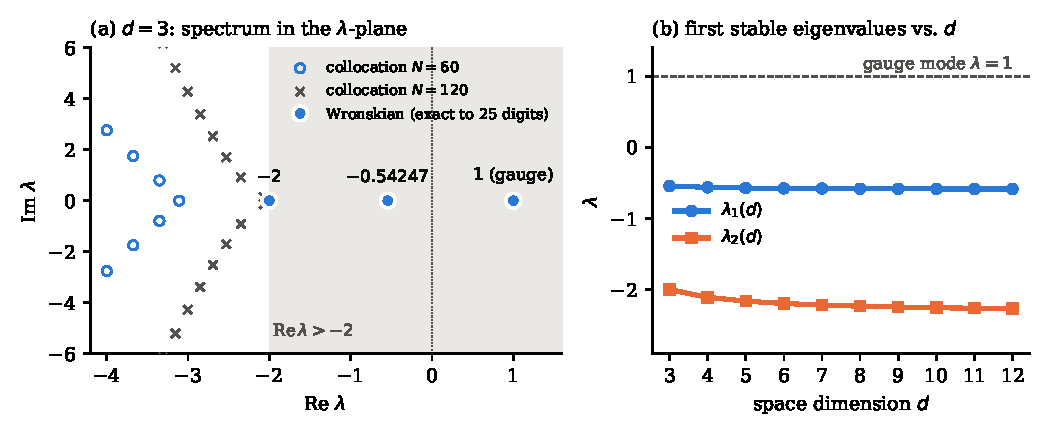
\includegraphics[width=\textwidth]{figures/geom_spectrum.pdf}
\caption{(a) $d=3$: collocation eigenvalues for $N=60$ (circles) and
$N=120$ (crosses) and the eigenvalues confirmed by the Wronskian (filled).
Collocation values with $\operatorname{Re}\lambda\lesssim-2$ move with $N$;
they come from the branch $(1-\rho^2)^{\sigma_2}$ with
$\operatorname{Re}\sigma_2\gtrsim3$, which polynomials cannot distinguish
from smooth functions at finite $N$, and they are rejected by the
Wronskian. They mirror the fact that on $\mathcal H_k$ the half-plane
$\operatorname{Re}\lambda<\frac d2-k$ is spectrum. (b) The first two stable
eigenvalues for $3\le d\le12$.}
\label{geom:fig:spec}
\end{figure}

\textbf{Findings (D).} (1) For $d=3,4,5$ the only eigenvalues in
$[-1.9,4]\times[-15,15]$ are the gauge mode and one real stable eigenvalue
$\lambda_1(d)$, and the only one in $[-2.25,-1.95]\times[-6,6]$ is
$\lambda_2(d)$ (argument principle); together with consequence~(i) of
\cref{geom:prop:hyp} for large real parts and the known exclusion of large imaginary parts
\cite{DonningerSchoerkhuberAichelburg2012} this is a numerical confirmation
of mode stability with spectral gap $|\lambda_1|$. (2) $\lambda_1(d)$
decreases slowly from $-0.5425$ ($d=3$) to $-0.5865$ ($d=12$). (3) For $d=3$,
$\lambda=-2$ is an eigenvalue with the explicit, analytic eigenfunction (in
the $u$-picture, $u-u_T\approx\varepsilon(T-t)^2\phi(\rho)$)
\[
  \phi(\rho)=\frac{3(1+\rho^2)^3\arctan\rho-3\rho-4\rho^3-9\rho^5}{\rho^2(1+\rho^2)},
\]
checked symbolically; here $\sigma_2=3$ and the Frobenius recursion at
$\rho=1$ turns out to be log-free, so $\rho=1$ imposes no condition. We know
no symmetry interpretation. (4) Consequently, in $\mathcal H_k$ with
$k>\frac d2+|\lambda_1|$, perturbations (after fixing $T$) should decay like
$e^{-\omega\tau}=(T-t)^{\omega}$ for every $\omega<|\lambda_1|$, i.e.\
$(T-t)^{0.54}$ for $d=3$. For $k=2$ and $d=3$ the free decay rate
$\omega_2=\frac12$ is the binding constraint, since $|\lambda_1|>\frac12$.

\subsection{Known stability theorems}
\label{geom:sec:wm-thm}

\begin{theorem}[\textbf{K}: Donninger \cite{Donninger2011};
Donninger--Sch\"orkhuber--Aichelburg \cite{DonningerSchoerkhuberAichelburg2012};
Costin--Donninger--Xia \cite{CostinDonningerXia2016}]\label{geom:thm:d3}
Let $d=3$. There are $\varepsilon,\delta>0$ such that for co-rotational data
$(u(0,\cdot),u_t(0,\cdot))$ that are $\varepsilon$-close to
$(f_0(r),rf_0'(r))$ (the profile with $T=1$) in a radial Sobolev norm of
sufficiently high regularity on the ball $\{r<1+\delta\}$, there is
$T\in(1-\delta,1+\delta)$ such that the solution blows up at $(T,0)$ and,
in similarity variables on the backward light cone of $(T,0)$, converges to
the profile $f_0$ exponentially in $\tau=-\log(T-t)$.
\end{theorem}
\cite{Donninger2011} proves this assuming mode stability,
\cite{DonningerSchoerkhuberAichelburg2012} develops the linear theory, and
\cite{CostinDonningerXia2016} proves mode stability, which makes the theorem
unconditional. Further results (all \textbf{K}):
\begin{itemize}[leftmargin=*,itemsep=1pt]
\item odd $d$: nonlinear stability of $f_0$
  \cite{ChatzikaleasDonningerGlogic2017}, using mode stability from
  \cite{CostinDonningerGlogic2017};
\item $d=3$, stability in the whole space (hyperboloidal similarity
  coordinates, evolution followed past the blowup time almost up to the
  Cauchy horizon) \cite{BiernatDonningerSchoerkhuber2021}; all $d\ge3$,
  global-in-space stability \cite{Glogic2025};
\item stability under perturbations small only in the critical Sobolev
  space: $d=4$ \cite{DonningerWallauch2023}; $d=3$, fractional critical space,
  via Strichartz estimates in similarity coordinates
  \cite{DonningerWallauch2025};
\item without any symmetry: mode stability for $d=3$
  \cite{WeissenbacherKochDonninger2025} and $d\ge4$
  \cite{DonningerMoscatelli2026a} (quasi-solution method with two extra
  parameters), and asymptotic stability \cite{DonningerMoscatelli2026b}
  (preprints). % TODO verify: dimension range and data space of DonningerMoscatelli2026b
\end{itemize}

\subsection{Relativistic membranes and the scalar Born--Infeld equation}
\label{geom:sec:membranes}

A timelike hypersurface $M^{d+1}\subset\mathbb{R}^{1,d+1}$ with vanishing
mean curvature (Nambu--Goto membrane; $d=1$ strings, $d=2$ membranes) is,
as a graph $z=u(t,x)$, a critical point of $-\int L$,
$L=\sqrt{1-u_t^2+|\nabla u|^2}$:
\begin{equation}\label{geom:eq:BI}
  \partial_t\Bigl(\frac{u_t}{L}\Bigr)-\nabla\!\cdot\!\Bigl(\frac{\nabla u}{L}\Bigr)=0
  \iff
  (1+|\nabla u|^2)u_{tt}-2u_t\nabla u\!\cdot\!\nabla u_t-L^2\Delta u+u_iu_ju_{ij}=0 ,
\end{equation}
the scalar Born--Infeld equation (the equivalence, after multiplication by
$L^3$, was checked in the radial case). It is quasilinear, hyperbolic
while $L^2>0$, and degenerates when $M$ becomes null. The scaling
$u\mapsto\mu^{-1}u(\mu t,\mu x)$ gives $s=-1$, so self-similar solutions are
$u=(T-t)U(x/(T-t))$: bounded slopes, curvature $\sim(T-t)^{-1}$.

\emph{Literature (K).} Eggers--Hoppe derived self-similar string solutions
in a graph representation near singularities (of swallowtail type) and their
extension to point singularities of membranes \cite{EggersHoppe2009};
Eggers--Hoppe--Hynek--Suramlishvili relate membrane singularities to
caustics of the eikonal equation and observe them numerically, e.g.\ at the
poles of collapsing ellipsoids \cite{EggersEtAl2015}. Nguyen--Tian show that
timelike maximal cylinders in $\mathbb{R}^{1+2}$ become singular in finite
time and, near a generic singularity, move rigidly or self-similarly
\cite{NguyenTian2013}. Wong proved that axially symmetric timelike minimal submanifolds (in the
class considered there) cannot exist globally in time, and analysed the
limiting geometry \cite{Wong2018}; Cai--Liu
construct radial singularities through loss of hyperbolicity (the surface
turns null) \cite{CaiLiu2025}. On the stability side,
Donninger--Krieger--Szeftel--Wong proved codimension-one stability of the
(static, non-singular) catenoid \cite{DonningerEtAl2016}, and
Bahouri--Marachli--Perelman constructed type~II blowup near the Simons cone,
adapting the Krieger--Schlag--Tataru method to this quasilinear setting
\cite{BahouriMarachliPerelman2021}. Yan proposed explicit ``lightlike''
self-similar solutions $u=\pm(T-t)\sqrt{1-\rho^2}$ and stability statements
in a proper subregion of the backward light cone
\cite{Yan2017,Yan2019b} (and for the $1{+}1$ Born--Infeld equation
\cite{Yan2019a}); see \cref{geom:prop:cone}(c) for what these solutions
are. We found no Donninger-type stability result for a \emph{timelike}
self-similar membrane singularity, nor for Born--Infeld blowup beyond
these preprints (literature search of October 2026, which had to stop
before every lead was exhausted).

\begin{proposition}[Self-similar membranes are minimal cones; \textbf{D}]
\label{geom:prop:cone}
Let $p=(T,0,0)$. Inside the backward light cone of $p$ the map
$(t,x,z)\mapsto(x,z)/(T-t)\in\mathbb{B}^{d+1}$ is the Beltrami--Klein model of
$\mathbb H^{d+1}$, and these are exactly the similarity coordinates.
\begin{enumerate}[label=(\alph*),leftmargin=*,itemsep=1pt]
\item The graph of $u=(T-t)U(\xi)$ is, inside the light cone of $p$, the
  cone $C(\Sigma)$ with vertex $p$ over
  $\Sigma=\{(\xi,U(\xi))\}\cap\mathbb{B}^{d+1}$; it solves
  \eqref{geom:eq:BI} iff $\Sigma$ is a minimal hypersurface of $\mathbb H^{d+1}$.
\item Normal perturbations $\varphi=\ell^{a}\chi(\omega)$, $\ell$ = proper
  time to $p$, solve the Jacobi equation $\Box_{C}\varphi+|\mathrm{II}_C|^2\varphi=0$
  iff $J_\Sigma\chi=(a-1)(a+d)\chi$, where
  $J_\Sigma=\Delta_\Sigma+|A_\Sigma|^2-d$ is the Jacobi operator of
  $\Sigma\subset\mathbb H^{d+1}$. In similarity variables $\lambda=1-a$:
  \[-J_\Sigma\chi=\lambda(d+1-\lambda)\chi .\]
  Translations give $\lambda=1$ ($\chi=\langle\nu,e\rangle$,
  $J_\Sigma\chi=-d\chi$); Lorentz transformations fixing $p$ give $\lambda=0$
  (Killing--Jacobi fields).
\item Consequences: for $d=1$ every self-similar string is a plane
  (geodesics of $\mathbb H^2$); every \emph{radial} self-similar graph regular at
  $\xi=0$ is $U\equiv c$, a plane moving with constant velocity (a minimal
  hypersurface of revolution meeting the axis is totally geodesic; the Taylor
  recursion of the radial ODE confirms $U''(0)=U^{(4)}(0)=\dots=0$ for
  $d=1,2,3$). The solutions $\pm(T-t)\sqrt{1-|x|^2/(T-t)^2}$ correspond to
  $\Sigma=\partial_\infty\mathbb H^{d+1}$: they satisfy the non-divergence
  form of \eqref{geom:eq:BI} but have $L\equiv0$, i.e.\ they are \emph{null}
  cones, where the equation is not hyperbolic (checked).
\end{enumerate}
\end{proposition}
\begin{proof}[Sketch]
The induced metric of $C(\Sigma)$ is $-d\ell^2+\ell^2g_\Sigma$, the radial
direction is geodesic and $\mathrm{II}_C=\ell\,\mathrm{II}_\Sigma$ on
$T\Sigma$, so $H_C=\ell^{-1}H_\Sigma$ and $|\mathrm{II}_C|^2=\ell^{-2}|A_\Sigma|^2$.
With $\Box_C=-\ell^{-d}\partial_\ell(\ell^d\partial_\ell)+\ell^{-2}\Delta_\Sigma$
one gets $(\Delta_\Sigma+|A_\Sigma|^2)\chi=a(a+d-1)\chi$, and
$\mathrm{Ric}_{\mathbb H^{d+1}}(\nu,\nu)=-d$. For $\Sigma=\mathbb H^d$ (the flat
membrane) this reproduces the free eigenvalues $\lambda\in\{1,0,-1,\dots\}$
of \cref{fw:sec} with $s=-1$, $V_0=0$. This is the membrane analogue of the
correspondence between self-similar wave maps and harmonic maps from
$\mathbb H^d$ \cite{CazenaveShatahTahvildarZadeh1998} and of
\cref{geom:prop:hyp}.
\end{proof}

\emph{Shrinking spheres (D).} A round $k$-sphere $R(t)\omega$ in
$\mathbb{R}^{k+1}$ ($k=1$ string, $k=2$ membrane) has Lagrangian
$-R^k\sqrt{1-R_t^2+|\nabla_{S^k}R|^2/R^2}$ (determinant of the induced metric
checked for $k=2$). Homogeneous solutions conserve
$E=R^k/\sqrt{1-\dot R^2}$; for $k=1$, $R=E\cos(t/E)$. Every such sphere
collapses at a finite time $T$ with $\dot R\to-1$ and Lorentz factor
$E/R^k\to\infty$:
\[
  R(t)=(T-t)-\frac{(T-t)^{2k+1}}{2(2k+1)E^2}+O\bigl((T-t)^{4k+1}\bigr).
\]
In similarity variables $R/(T-t)\to1$: the collapse is \emph{lightlike}; the
limiting profile is the null cone of \cref{geom:prop:cone}(c), sitting on the
boundary $|\xi|=1$ of the similarity domain. Linearising about it,
$R=R_0+\varepsilon\sum\delta_{\ell}(t)Y_{\ell}$ gives (derived and checked)
\begin{equation}\label{geom:eq:sphere-lin}
  \ddot\delta_\ell-2k\frac{\dot R_0}{R_0}\dot\delta_\ell
  +\frac{\ell(\ell+k-1)-k}{E^2}R_0^{2k-2}\delta_\ell=0 ,
\end{equation}
whose exponents at $t=T$ are $0$ and $2k+1$. Hence generically
$\delta_\ell(T)\ne0$ and $\delta_\ell/R_0\sim(T-t)^{-1}$: in similarity
variables \emph{every} harmonic $(\ell,m)$ has a mode with $\lambda=1$ (and
one with $\lambda=-2k$). Only $\ell=0$ (time shift) and $\ell=1$
(translations) are symmetries; for instance, for $k=2$, $E=1$, data
$(\delta_\ell,\dot\delta_\ell)=(0,1)$ at rest we find
$\delta_\ell(T)=0.5,\,0.437,\,0.328,\,0.2,\,0.083$ for $\ell=0,\dots,4$
(\texttt{geom\_membrane.py}). Geometrically, each ray of the
ultra-relativistic membrane reaches the centre at its own time: the round
focus is an infinitely degenerate caustic which generic perturbations
unfold, in line with the caustic picture of \cite{EggersEtAl2015}. Spherical
collapse is therefore unstable in infinitely many directions, and a
Donninger-type argument (finite-dimensional instabilities removed by
modulation) cannot apply to it.

\subsection{Assessment and open problems}
\label{geom:sec:assess}

\begin{enumerate}[leftmargin=*,itemsep=2pt]
\item \textbf{Wave maps (K + D).} The Donninger programme is complete for
  co-rotational wave maps into $S^d$, $d\ge3$, and is now being extended
  beyond symmetry. Our computations reproduce the spectral picture
  (gauge mode $\lambda=1$, gap $|\lambda_1|\approx0.54$--$0.59$), give a
  self-contained proof of the absence of eigenvalues with
  $\operatorname{Re}\lambda\ge\frac{d-1}{2}$ other than the gauge mode for $d=3$
  (consequence~(i) of \cref{geom:prop:hyp}), and give an explicit SUSY partner
  \eqref{geom:eq:susy}. The open cases relevant for applications are $d=2$
  with target $S^2$ (bubbling, not self-similar, so a different theory) and
  $d=3$ with target $S^2$, where neither the profile nor its stability is
  settled as far as we know.
\item \textbf{Membranes: obstacles (D).} (a) \emph{Quasilinearity:} the
  perturbation $\mathbf L'$ contains second derivatives, so it is not compact
  relative to $\mathbf L_0$, and the domain of dependence moves with the
  solution. One needs energy estimates adapted to the background's
  characteristic cone; this has not been done in similarity variables.
  (b) \emph{Characteristic degeneracy:} the singularities found so far in
  analysis and numerics (strings, spheres, axisymmetric membranes) are
  lightlike, and then the
  similarity variables put the profile on the boundary $|\xi|=1$. (c)
  \emph{Gauge:} the graph gauge fails where the surface turns vertical
  (swallowtails); normal graphs over the cone are the natural choice in
  \cref{geom:prop:cone}.
\item \textbf{Where a Donninger-type theory is plausible (C).} Timelike
  self-similar membranes are cones over minimal hypersurfaces
  $\Sigma\subset\mathbb H^{d+1}$. Such $\Sigma$ with prescribed ideal
  boundary exist in abundance by classical results on the asymptotic
  Plateau problem in hyperbolic space.
  % TODO verify refs: Anderson (asymptotic Plateau problem); Hardt--Lin (regularity at infinity)
  The questions are whether some non-flat $\Sigma$ extends
  \emph{smoothly} across the ideal boundary in the Klein coordinates, i.e.\
  across the light cone of $p$, which is the analogue of the selection of
  $f_0$ by smoothness at $\rho=1$, and whether the resonances of $J_\Sigma$
  in \cref{geom:prop:cone}(b) satisfy mode stability. Boundary expansions of
  minimal submanifolds in hyperbolic space suggest that a generic $\Sigma$
  has a non-smooth term of order $(1-|\xi|^2)^{(d+1)/2}$ (with a logarithm
  for odd $d$), so smooth cones, if they exist, are isolated. We have not
  verified this.
\item \textbf{Industrial relevance (honest).} Nambu--Goto and Born--Infeld
  are physics models (strings and branes, nonlinear electrodynamics). The
  engineering large-deflection membrane
  $\rho_h u_{tt}=\mathcal T\,\nabla\!\cdot(\nabla u/\sqrt{1+|\nabla u|^2})$
  shares the scaling $s=-1$ but is not Lorentz invariant and is hyperbolic
  for every slope, with squared wave speeds
  $\mathcal T/(\rho_h W)$ and $\mathcal T/(\rho_h W^3)$, $W=\sqrt{1+|\nabla u|^2}$,
  so there is no null degeneration (the speeds degenerate only as
  $|\nabla u|\to\infty$). We know of no self-similar blowup result
  for it; in MEMS the dominant membrane nonlinearity is usually stretching,
  not slope.
\end{enumerate}
